\documentclass[11pt,a4paper]{article}
\usepackage{fontspec}
\usepackage{polyglossia}\setdefaultlanguage{slovenian}

\usepackage[margin=2.2cm]{geometry}
\usepackage{graphicx,booktabs,longtable,amsmath,amssymb,array,float,caption,xcolor}
\usepackage{needspace}
\usepackage[hidelinks]{hyperref}
\renewcommand{\figurename}{Slika}
\renewcommand{\tablename}{Tabela}
\gappto\captionsslovenian{\renewcommand{\refname}{Viri}\renewcommand{\abstractname}{Povzetek}\renewcommand{\figurename}{Slika}}
\renewcommand{\topfraction}{0.9}\renewcommand{\bottomfraction}{0.8}\renewcommand{\textfraction}{0.1}\renewcommand{\floatpagefraction}{0.75}\setcounter{topnumber}{3}
\renewcommand{\abstractname}{Povzetek}
\definecolor{capc}{HTML}{4A2A6B}\captionsetup{font={small,color=capc},labelfont=bf,margin=1.2cm,justification=centering}
\setlength{\parskip}{0.4em}
\setlength{\parindent}{0pt}
\setlength{\emergencystretch}{3em}

\newcommand{\repo}{\url{https://github.com/timkmecl/referendumi-2026-analiza}}

\title{Sum na zamenjavo glasov ZA in PROTI\\na posameznih voliščih referendumov 2026\\[0.3em]\large Krajša predstavitev analize}
\author{Tim Kmecl, dipl. inž. rač. in mat.}
\date{15.~oktober 2026}

\begin{document}
\begin{center}
{\LARGE Sum na zamenjavo glasov ZA in PROTI\\[0.15em]na posameznih voliščih referendumov 2026\par}
\vspace{0.3em}{\large Krajša predstavitev analize\par}
\vspace{0.4em}{\large Tim Kmecl, dipl. inž. rač. in mat.}\quad{\small 15.~oktober 2026}\par
\vspace{0.2em}{\footnotesize Celotno poročilo, koda in podatki: \repo\par}
\end{center}
\vspace{-0.6em}
\begin{center}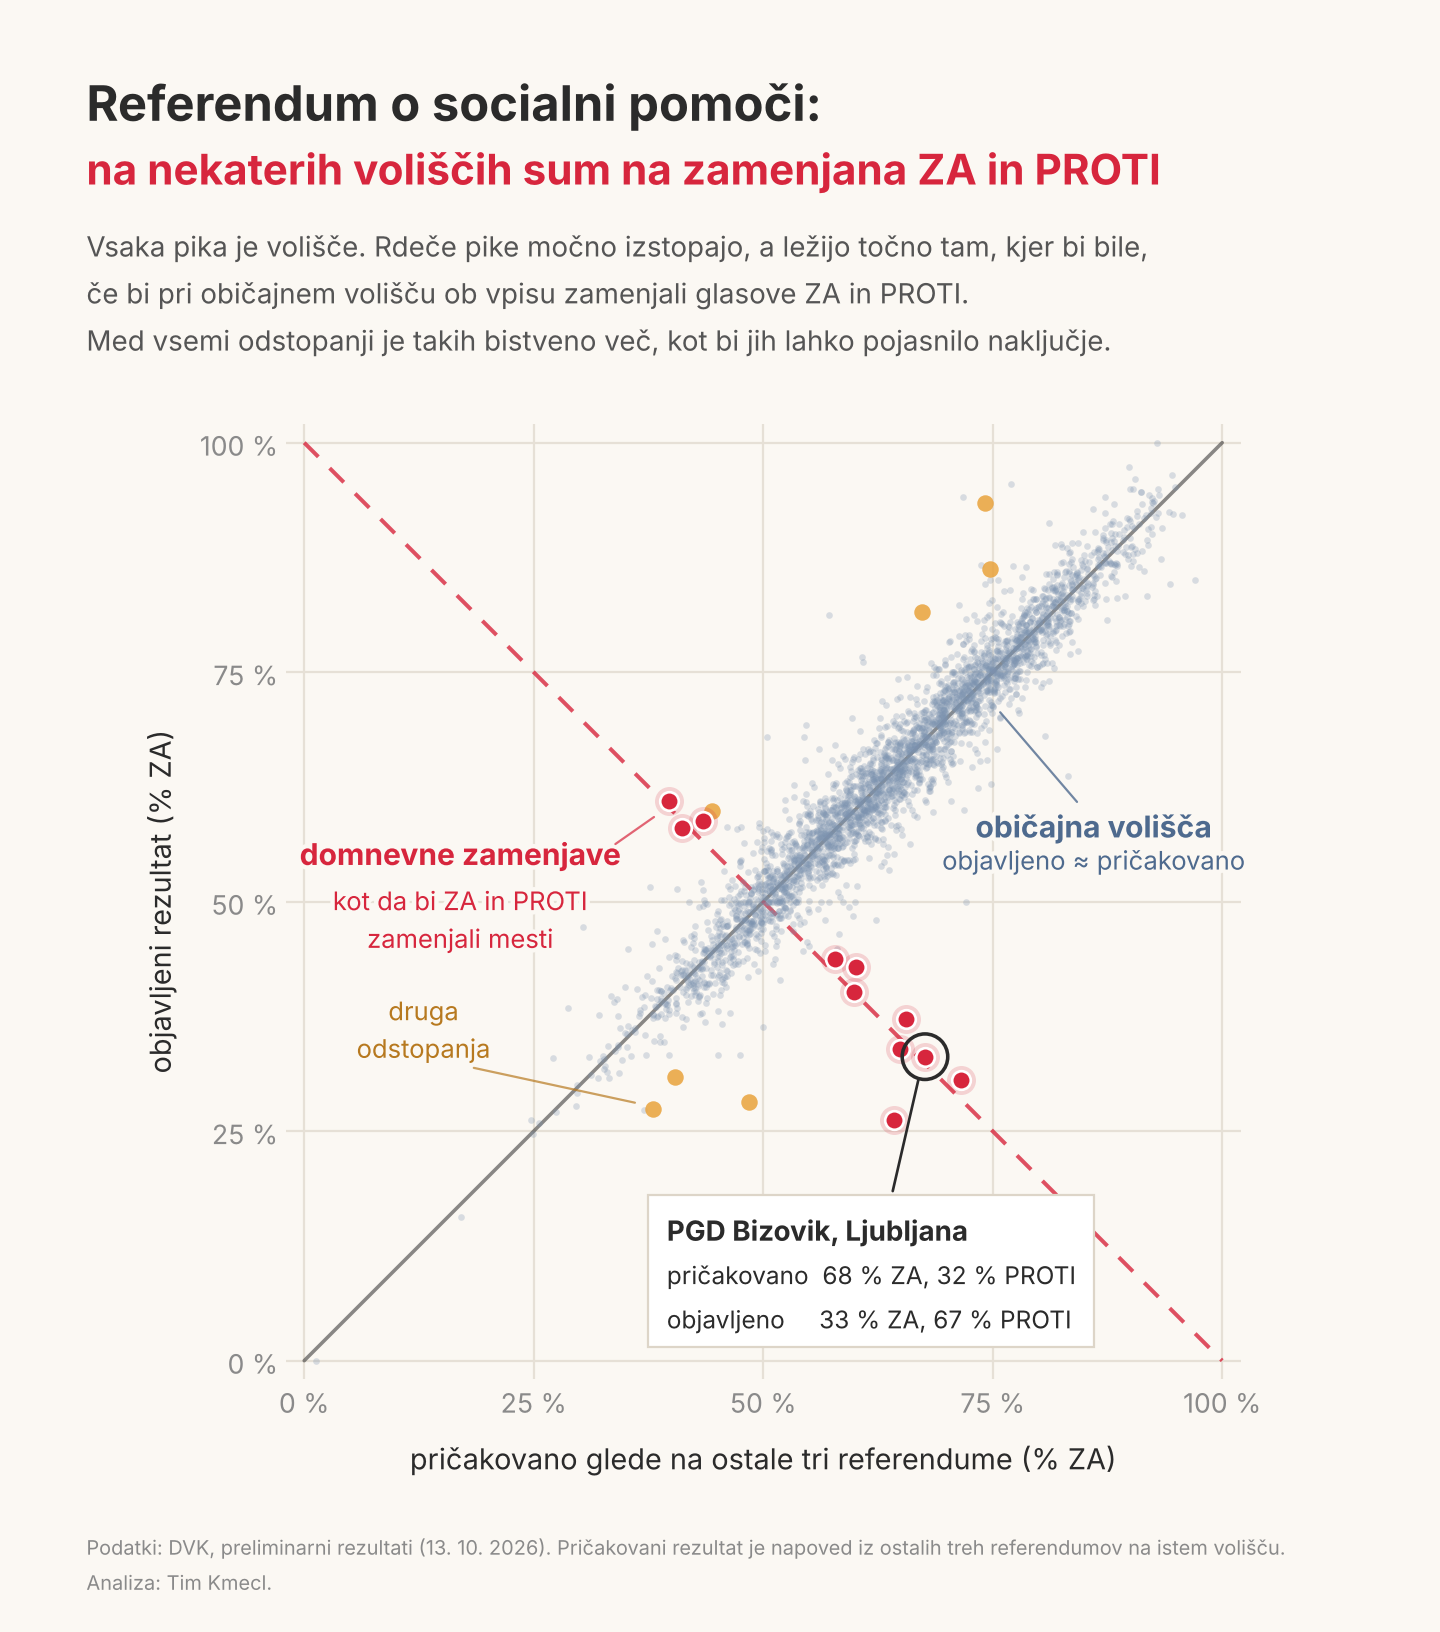
\includegraphics[height=0.4\textheight]{javnost_sociala.png}\end{center}
\vspace{-0.8em}
{\small
\begin{center}\textbf{Povzetek}\end{center}\vspace{-1.2em}
\setlength{\parskip}{0.4em}
Ker na istem volišču glasujejo isti volivci, je mogoče rezultat vsakega od štirih sočasnih referendumov z visoko natančnostjo napovedati iz preostalih treh. Med 12\,760 rezultati (3190 volišč $\times$ 4 referendumi) jih 53 od napovedi odstopa za več kot pet standardnih odklonov ($|z|>5$). \textbf{Ključni argument ni sam obstoj izstopajočih rezultatov} (njihovo število bi lahko pojasnile resnične lokalne posebnosti, porazdelitev z debelejšimi repi od predpostavljene ali nenatančnost modela), \textbf{temveč \emph{kje} ležijo: statistično izrazito se zgoščajo na zrcalni vrednosti napovedi ($\boldsymbol{100-\hat p}$).} V pas okoli nje pade 27 od 53, ob naključnih odstopanjih bi jih pričakovali 7--9 ($p\approx10^{-7}$--$10^{-8}$). Znotraj njega se kopičijo v še ožjem pasu okoli zrcalne vrednosti ($\pm1$ standardni odklon), kot to velja za binomski šum okoli pravega rezultata: 17, pričakovano 2,5.

Nobena od nedolžnih razlag ne napoveduje vrha na točno določeni vrednosti. Resnična posebnost premakne rezultat za količino, ki ni povezana z oddaljenostjo napovedi od 50~\%, debelejši repi in nenatančen model pa porazdelitev odstopanj le razširijo. Zrcalna vrednost je za vsako volišče drugačna, zato bi se morala vsaka nedolžna razlaga nanjo ``uglasiti'' na vsakem volišču posebej. Resnična posebnost bi se poleg tega praviloma pokazala tudi na sosednjih voliščih v isti stavbi, a pri sedmih od osmih takih primerov se ne. \textbf{Najverjetnejša razlaga je administrativna zamenjava števil ZA in PROTI pri vpisu ali prepisu}, ocenjeno pri okoli 22 rezultatih. S tem so skladne tudi ostale značilnosti: smer odstopanj je skladna z naključjem, geografskega vzorca ni, zamenjave pa so pogostejše na večjih voliščih, približno sorazmerno s številom glasov, kar ustreza človeški napaki pri štetju in vpisu. Nobena značilnost podatkov ne kaže na sistematično prirejanje.

Takšne napake niso brez precedensa. Na Danskem so leta 2014 s primerjavo sočasnega referenduma in volitev po voliščih odkrili volišče z zamenjanima ZA in PROTI, kar je volilni organ še isti dan potrdil. Revizija novozelandskih volitev 2023 pa je napake pri vnosu rezultatov odkrila na 0,3--0,7~\% volišč. \textbf{Domnevne napake ne spremenijo izida nobenega referenduma}; največji učinek bi imele pri RTV, kjer bi se prednost PROTI povečala s 546 na okoli 1400 glasov. Statistika napake na posameznem volišču ne more dokazati, hipotezo pa je \textbf{enostavno preveriti}: pregled zapisnikov in glasovnic na treh voliščih z najmočnejšim signalom bi jo z veliko zanesljivostjo potrdil ali ovrgel.\par}



%=====================================================
\section{Podatki in izhodišče}

Analizirani so preliminarni rezultati po voliščih za štiri sočasne referendume (parlamentarna preiskava, RTV, sociala, tujci), preneseni s spletne strani Državne volilne komisije 13.\,10.\,2026 ob 19:30. Gre za \textbf{preliminarne in ne uradne rezultate}: glasovi po pošti iz tujine so povsod 0, DVK pa je lahko katero od navedenih volišč medtem že popravila. Vključena so volišča z vsaj 10 veljavnimi glasovi pri vseh štirih referendumih (3190 volišč, vključno s predčasnim glasovanjem).

\begin{center}
\small\begin{tabular}{lrrr}
\toprule
Referendum & ZA \% & razlika (glasovi) & zmagovalec \\
\midrule
Parlamentarna preiskava & 48,74 & 23\,147 & PROTI \\
RTV & 49,97 & 546 & PROTI \\
Sociala & 60,54 & 194\,705 & ZA \\
Tujci & 55,30 & 97\,776 & ZA \\
\bottomrule
\end{tabular}
\end{center}

\textbf{Opomba o izrazih.} Analiza je statistična in temelji le na objavljenih številih. Kjer zaradi jedrnatosti piše ``napaka'' ali ``zamenjava'', je vedno mišljena \emph{domnevna} napaka oziroma \emph{sum na} zamenjavo: volišče, katerega objavljeni rezultat se statistično ujema z vzorcem zamenjave. Ali je napaka dejansko nastala, je mogoče ugotoviti le s pregledom zapisnikov in glasovnic.

\subsection{Podobni primeri in metode}

Zamisel, da rezultate na volišču preverimo z rezultati drugih glasovanj na istem volišču, ni nova. Wand in sod.~\cite{wand2001} so po voliščih primerjali glasove za kandidata Buchanana na predsedniških volitvah v ZDA leta 2000 z glasovi za druge tekme na isti glasovnici in pokazali, da je nenavadno visok delež v okrožju Palm Beach posledica zmedne oblike glasovnice, ne pa dejanske podpore volivcev. Robustne regresijske metode za odkrivanje izstopajočih števil glasov po voliščih sta razvila Mebane in Sekhon~\cite{mebane2004}.

Najbližji precedens je primer z Danske: na dan evropskih volitev 2014 je potekal tudi referendum o Enotnem patentnem sodišču, aktivisti organizacije Open Knowledge Denmark pa so po voliščih primerjali glasove ZA na referendumu z glasovi za stranke, ki so zagovarjale PROTI. Eno volišče (okoli 800 glasov) je izrazito izstopalo; volilni uradnik je še isti dan potrdil, da sta bila ZA in PROTI zaradi človeške napake zamenjana~\cite{okfn2014}. Napake pri vnosu se pojavljajo tudi v sistemih z razvitimi kontrolami: revizija novozelandskih volitev 2023 je na okoli 0,3--0,7~\% volišč odkrila napake, pri katerih so bili glasovi vpisani napačnim kandidatom ali strankam ali pa sta bila zamenjana rezultata predčasnega glasovanja in volilnega dne~\cite{oagnz2024}. Ahlbäck in Jablonski~\cite{ahlback2025} sta na volitvah v Malaviju 2019 pokazala, da je bila večina popravkov v zapisnikih volišč posledica človeških napak in ne prevar ter da njihovo število narašča z zahtevnostjo štetja.

%=====================================================
\section{Model}

\subsection{Zakaj štirje referendumi}

Na istem volišču glasujejo isti volivci o štirih vprašanjih. Deleži ZA so med volišči močno povezani: uteženi korelacijski koeficienti so 0,95--0,98, in tudi znotraj istega volilnega okraja (po odštetju povprečja okraja) ostanejo 0,93--0,96. Volišče je torej samo sebi najboljša referenca: rezultat enega referenduma lahko napovemo iz ostalih treh veliko natančneje kot iz povprečja okraja.

Ključna lastnost: splošni lokalni premik (``bolj levo'' ali ``bolj desno'' volišče) se pokaže pri vseh štirih referendumih hkrati in se v napovedi izniči. Napaka v zapisniku ali pri vnosu pa prizadene en sam referendum.

\subsection{Napoved}

Za vsak referendum $k$ in volišče $i$ ocenim regresijo v logitih ($\operatorname{logit}p=\ln\frac{p}{1-p}$):
\begin{equation}
\operatorname{logit}\hat p_{ik} = \beta_{0k} + \sum_{j\neq k}\beta_{jk}\,\operatorname{logit} p_{ij},
\label{eq:model}
\end{equation}
kjer je $p_{ij}$ objavljeni delež ZA na volišču $i$ pri referendumu $j$ in $\hat p_{ik}$ napoved za referendum $k$. Uteži so $w_{ik}=n_{ik}\,p_{ik}(1-p_{ik})$ (inverzna varianca deleža, $n_{ik}$ je število veljavnih glasov). Ocena je robustna (Huberjeva funkcija izgube), da izstopajoče vrednosti ne vplivajo na koeficiente. Model ocenim dvakrat, brez in s fiksnimi učinki okraja (dodaten člen za vsak okraj); oba dajeta skoraj enake rezultate.

\textbf{Dvostopenjsko čiščenje.} Napovedovalci so lahko tudi sami napačni: napaka pri preiskavi bi pokvarila napoved za ostale tri referendume. Zato najprej izračunam robustno predhodno napoved (mediano treh modelov z enim napovedovalcem, ki je ena sama napaka ne more premakniti) in na volišču z izrazitim odstopanjem celico z največjim odstopanjem nadomestim s predhodno napovedjo, vendar \emph{samo v vlogi napovedovalca}. Končna napoved je polni model s tremi napovedovalci na očiščenih podatkih. Odstopanje vsake celice je vedno izračunano iz \emph{objavljenega} deleža in napovedi iz ostalih treh referendumov.

\textbf{Preverjanje krožnosti.} Ker predhodna napoved posredno vsebuje informacijo o vseh referendumih, bi lahko napoved rahlo potegnila k objavljeni vrednosti (kar bi bilo konzervativno). Postopek sem zato ponovil tako, da nadomestna vrednost pri napovedi referenduma $j$ ne uporablja $j$. Množica izstopajočih celic in domnevnih zamenjav ostane popolnoma enaka.

\subsection{Odstopanje in natančnost}

Odstopanje objavljenega deleža od napovedi in odstopanje, ki bi ga dobili po zamenjavi ZA in PROTI, merim v enotah šuma:
\begin{equation}
z_{ik} = \frac{p_{ik}-\hat p_{ik}}{c_k\sqrt{\hat p_{ik}(1-\hat p_{ik})/n_{ik}}},\qquad
z^{\text{zam}}_{ik} = \frac{(1-p_{ik})-\hat p_{ik}}{c_k\sqrt{\hat p_{ik}(1-\hat p_{ik})/n_{ik}}}.
\label{eq:z}
\end{equation}
Imenovalec je binomski šum, ki upošteva velikost volišča. Faktor $c_k$ je robustna ocena dejanske razpršenosti iz podatkov in znaša 0,69--1,01, večinoma okoli 0,8. Vrednost pod 1 pomeni, da je napoved natančnejša od binomskega šuma med neodvisnimi vzorci. To je pričakovano, saj na vseh štirih referendumih glasujejo \emph{isti} volivci in del naključnosti (kdo je prišel na volišče) je skupen vsem štirim. Ker je $c_k$ ocenjen iz podatkov, šum ni podcenjen.

Napoved pojasni 95--98~\% razlik med volišči (utežen $R^2$), tipično odstopanje objavljenega deleža od napovedi pa je 2--3 odstotne točke (mediana absolutnega odstopanja 1,5--2 o.\,t.). To je primerljivo z binomskim šumom zaradi končnega števila volivcev, zato ni pričakovati, da bi bila napoved lahko bistveno natančnejša.

Celico (volišče $\times$ referendum) z $|z|>5$ v obeh modelih imenujem \textbf{outlier}. Outlier, ki se po zamenjavi ZA in PROTI ujema z napovedjo ($|z^{\text{zam}}|<3$ v obeh modelih), je \textbf{domnevna zamenjava}.

%=====================================================
\section{Rezultati}

Jedro porazdelitve $z$ je pri vseh štirih referendumih normalno, outlierji pa tvorijo ločen rep (slika~\ref{fig:qq}, levo). Po Gaussovi porazdelitvi bi pričakovali manj kot 0,01 celice z $|z|>5$, opaženih je 53 (na 50 voliščih). Outlierji niso posledica majhnih volišč: večinoma so na voliščih s 100--1000 glasovi, kjer je šum majhen (slika~\ref{fig:qq}, desno). Pri vseh je število oddanih glasovnic med štirimi referendumi skladno, zato je odstopanje v razdelitvi glasov na ZA in PROTI, ne v številu glasovnic.

\begin{figure}[H]
\centering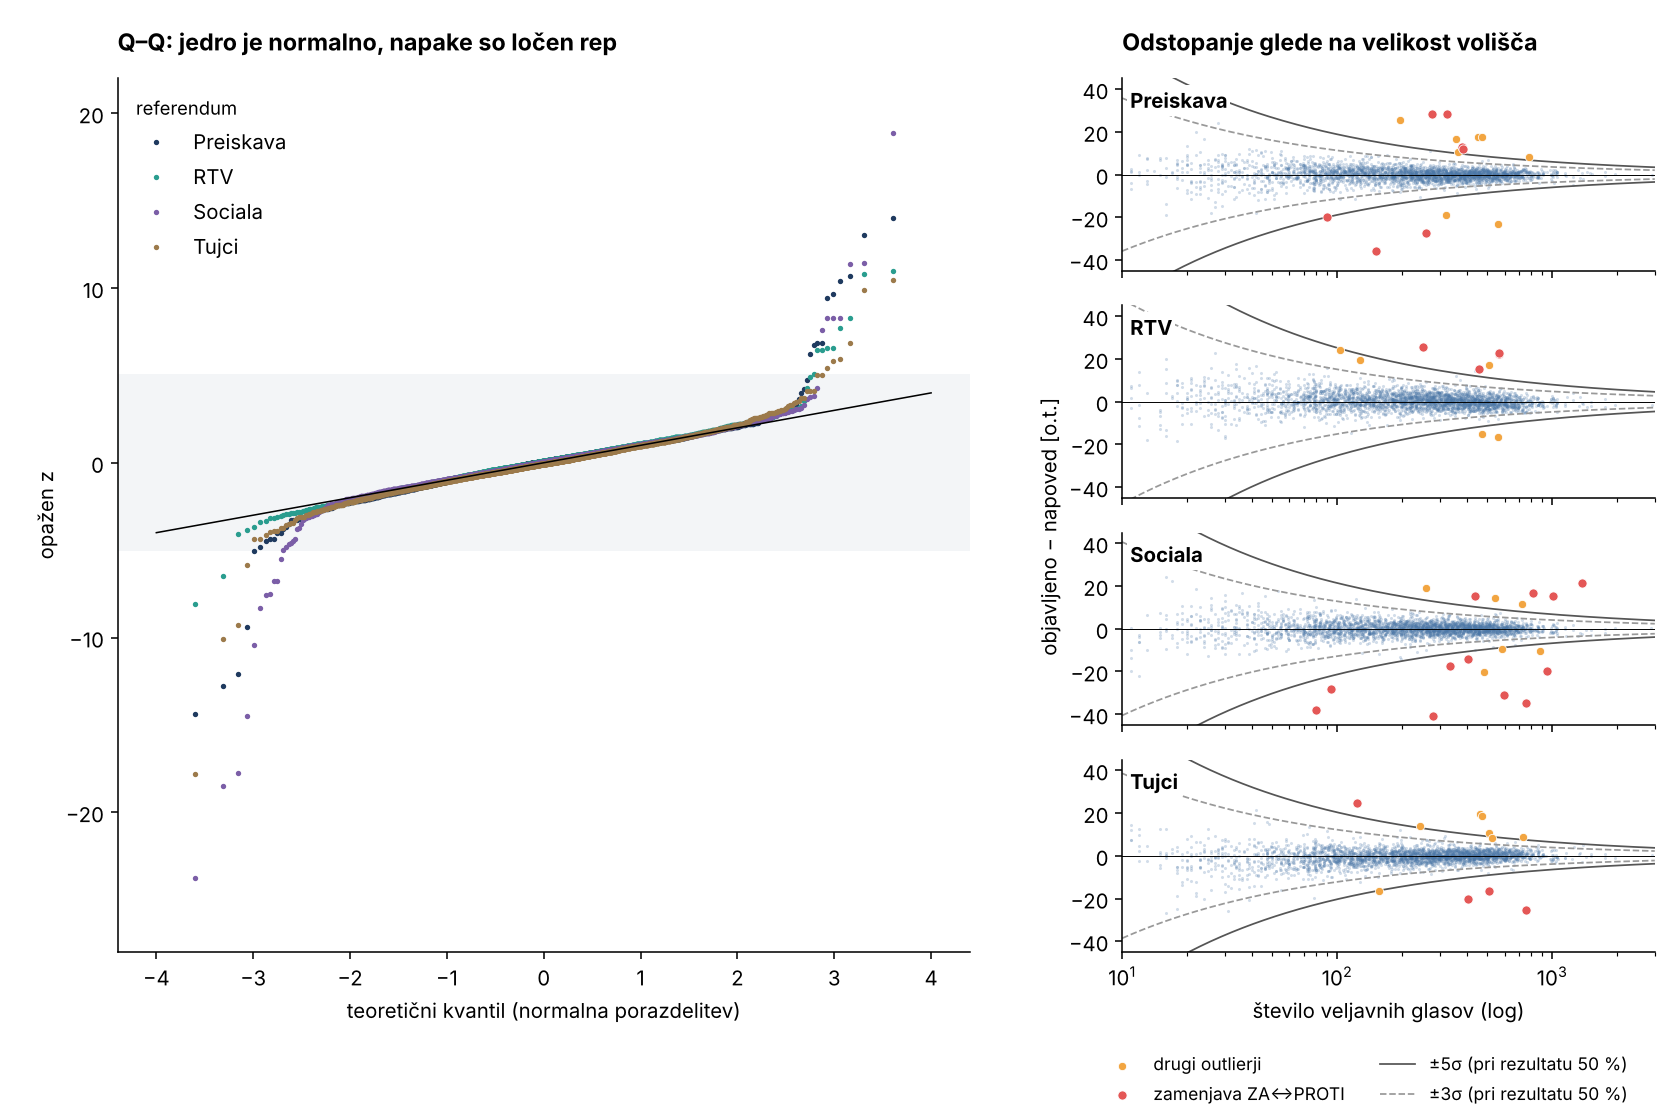
\includegraphics[width=0.9\textwidth]{4_qq_lijak.png}
\caption{Levo: Q--Q diagram odstopanj $z$. Desno: odstopanje od napovedi glede na velikost volišča.}
\label{fig:qq}
\end{figure}

Slika~\ref{fig:napoved} kaže objavljeni rezultat proti napovedi za vse štiri referendume. Normalna volišča ležijo na diagonali, volišče z zamenjanima ZA in PROTI pa bi ležalo na zrcalni črti, objavljeno $=100-$napoved. Outlierji se zgoščajo ob zrcalni črti pri vseh štirih referendumih, najizraziteje pri sociali (slika na prvi strani).

\begin{figure}[H]
\centering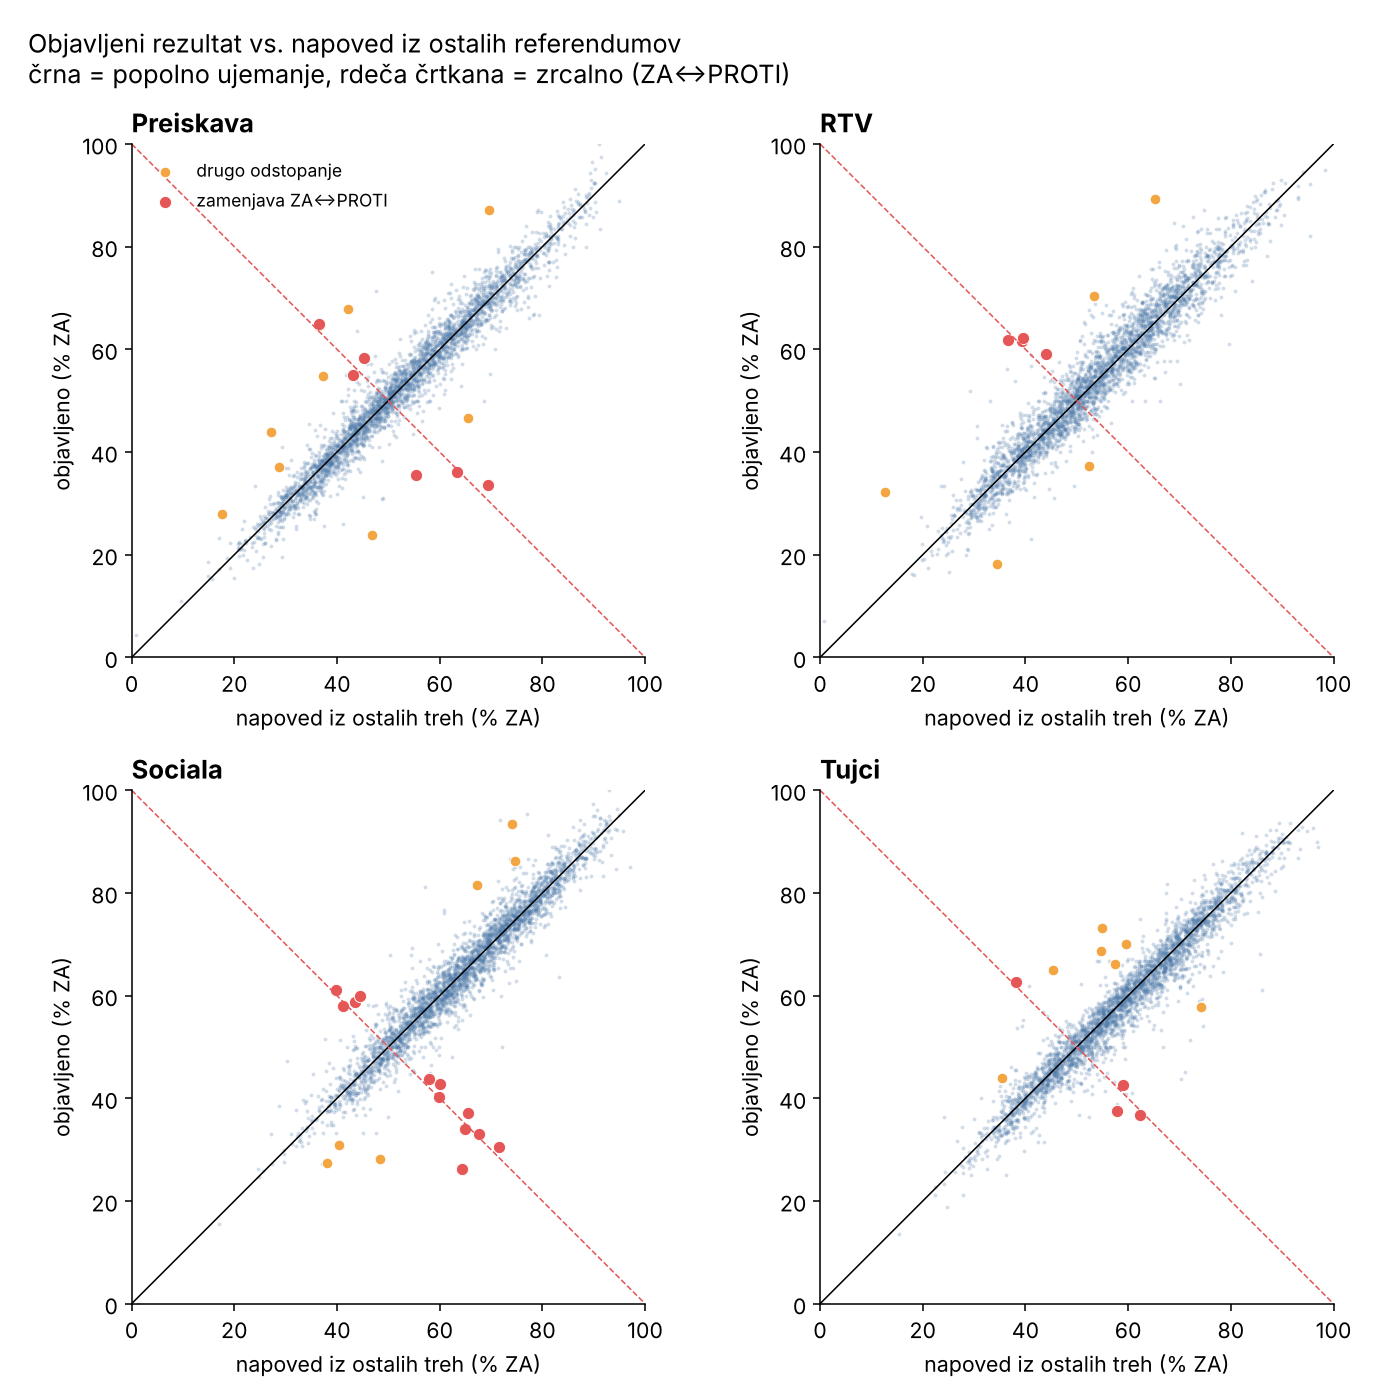
\includegraphics[width=0.6\textwidth]{1_napoved_vs_objavljeno.png}
\caption{Objavljeni proti napovedanemu deležu ZA, vsi štirje referendumi.}
\label{fig:napoved}
\end{figure}

Od 53 outlierjev jih je 26 domnevnih zamenjav (preiskava 7, RTV 4, sociala 11, tujci 4), 1 morda zamenjava, 5 celic na dveh voliščih z odstopanjem pri več referendumih in 21 nepojasnjenih. Razliko med vrstami najbolje pokažejo ``prstni odtisi'' posameznih volišč (slika~\ref{fig:prst}). Za vsak referendum je prikazan objavljeni delež ZA (poln krog), njegova zrcalna vrednost (prazen krog) in napoved iz ostalih treh referendumov s pasom $\pm3$ standardne odklone. Na tipičnem volišču (Bežigrad~2/8) so vsi objavljeni rezultati v pasu. Pri Kopru~1/22 in Viču/31 izstopa en referendum, njegova zrcalna vrednost pa pade točno na napoved. Pri Škofji Loki~1/6 izstopata dva referenduma in zamenjava ne pomaga. Pri Muljavi izstopa en referendum, vendar stran od 50~\%, zato ga zamenjava ne pojasni.

\begin{figure}[H]
\centering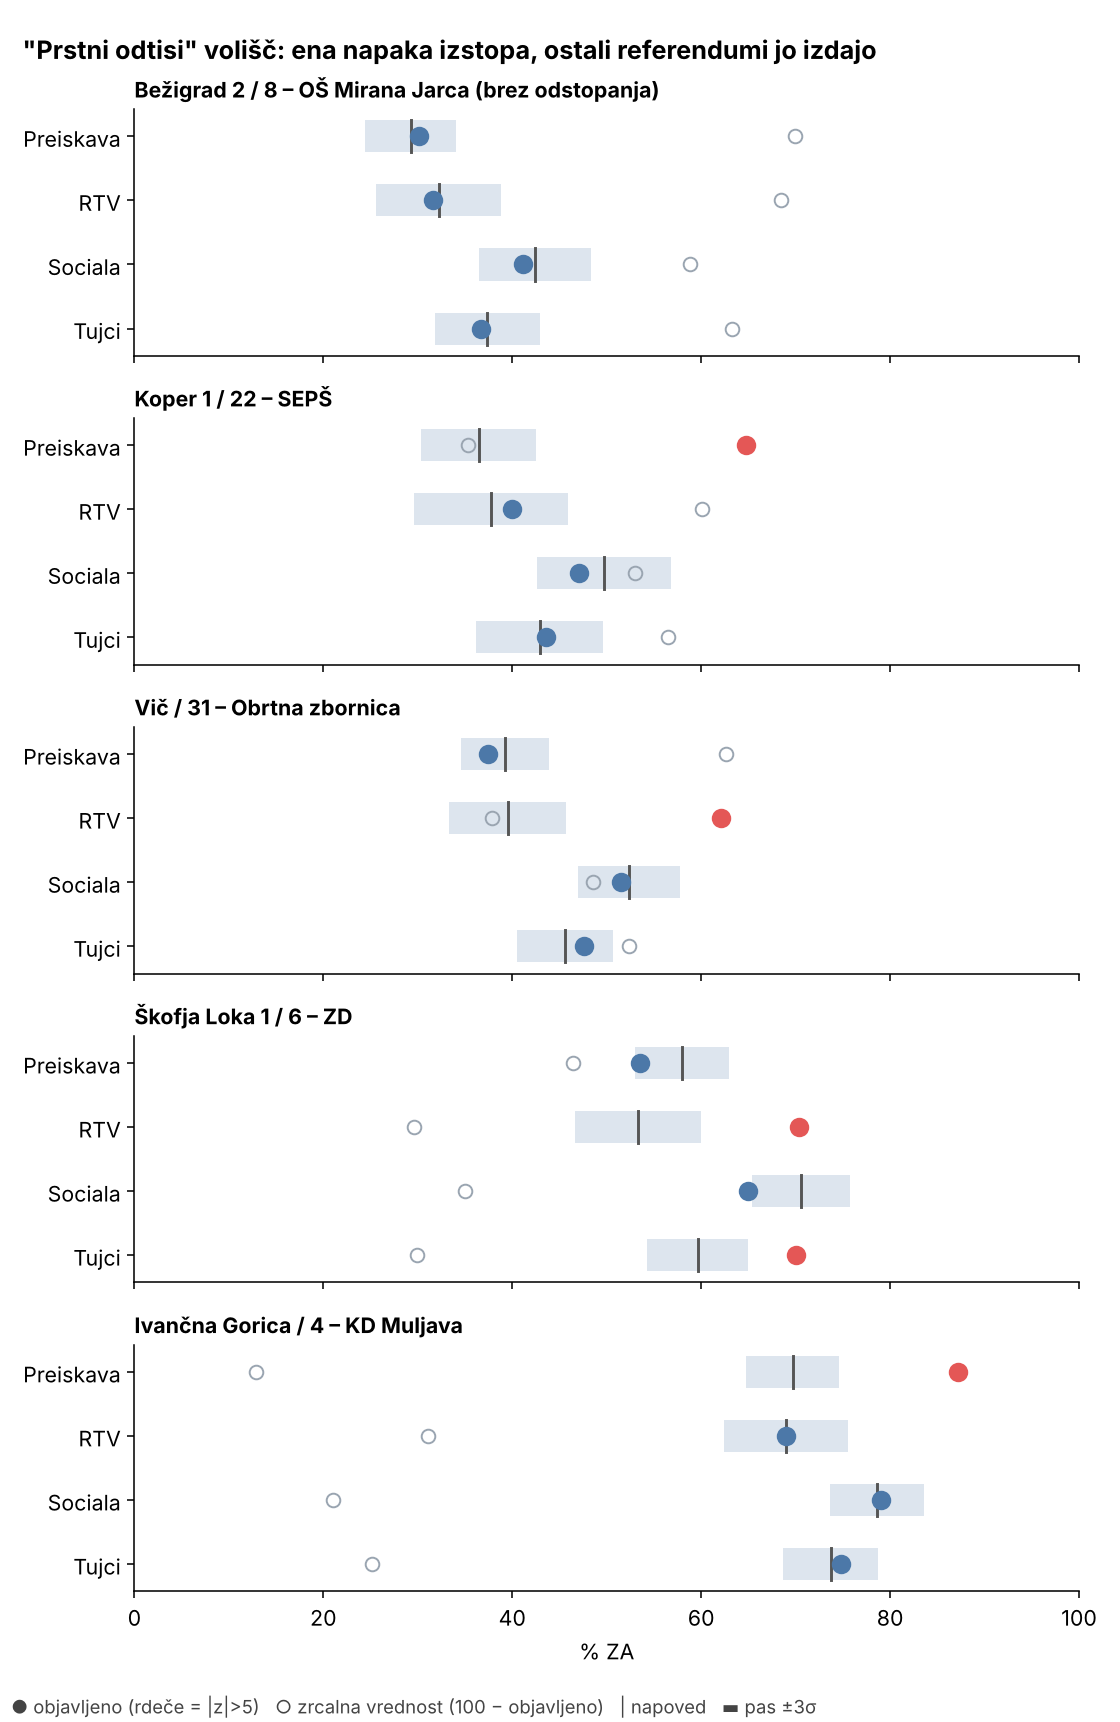
\includegraphics[width=0.56\textwidth]{3_prstni_odtisi.png}
\caption{``Prstni odtisi'' petih volišč.}
\label{fig:prst}
\end{figure}

%=====================================================
\section{Ali gre res za napake?}

Ključno vprašanje je, ali je sum na napake upravičen, ali pa so outlierji brez napak: posledica resničnih, morda zelo izrazitih posebnosti volišč, ali pa so odstopanja porazdeljena z debelejšimi repi od predpostavljene normalne porazdelitve. Sam kriterij $|z^{\text{zam}}|<3$ ni dokaz: pri volišču z napovedjo blizu 50~\% je zrcalna vrednost blizu objavljene, zato v pas lahko pade tudi resnično odstopanje.

\subsection{Diagnostični diagram}

Za vsako celico velja $z - z^{\text{zam}} = (1-2\hat p)/\text{šum}$, razlika med njima je torej razdalja napovedi od 50~\% v enotah šuma. Normalne celice so v pasu $|z|<5$, kjer $z^{\text{zam}}$ niha poljubno. Domnevne zamenjave so outlierji v vodoravnem pasu $|z^{\text{zam}}|<3$, drugi outlierji pa so razpršeni zunaj njega (slika~\ref{fig:diag}). Že na sliki je vidno, da outlierji ne sledijo razporeditvi normalnih točk. Navpični položaj normalnih točk je razpršen od približno $-40$ do $+30$, pas $|z^{\text{zam}}|<3$ pa jih vsebuje le majhen del. Med outlierji pa jih v tem ozkem pasu leži približno polovica. Ali je to zgoščevanje res večje, kot bi ga dala naključna odstopanja, preverim v nadaljevanju.

\begin{figure}[H]
\centering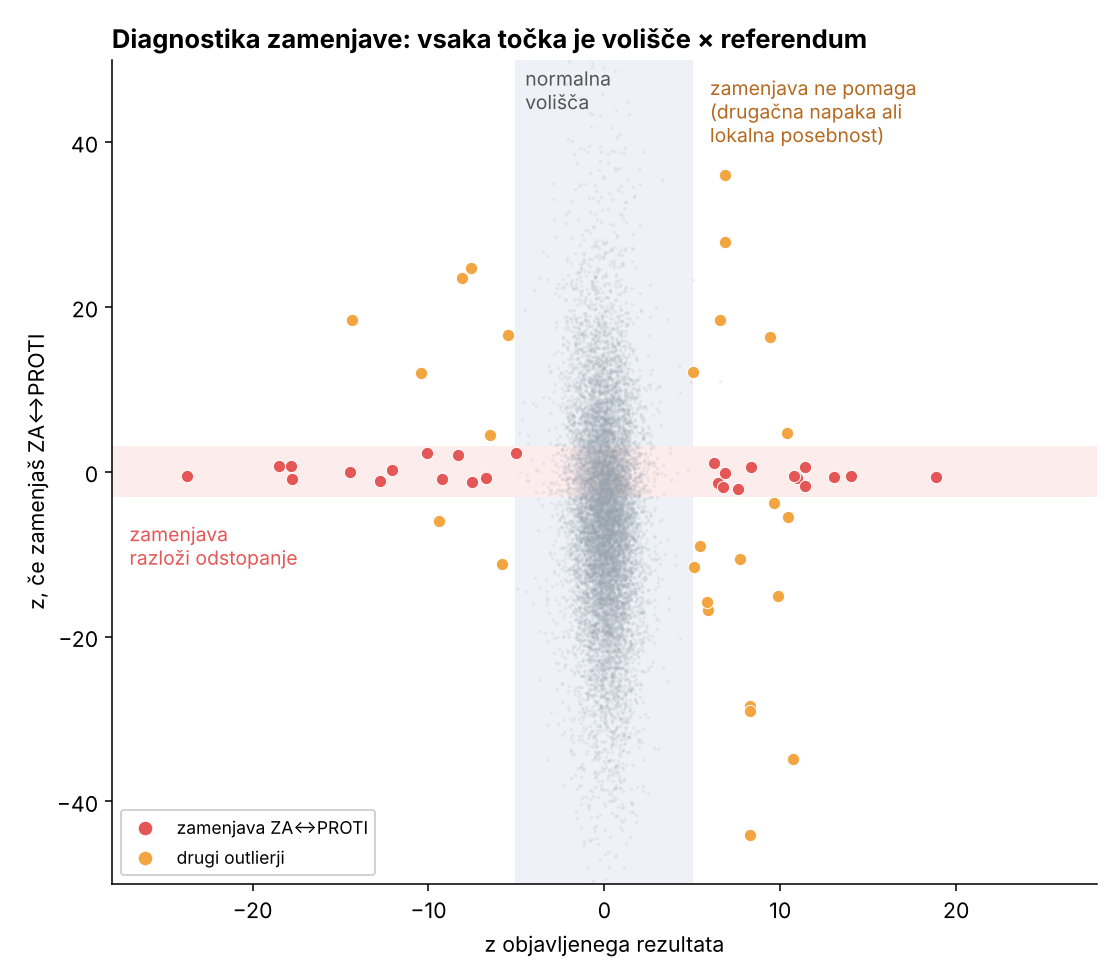
\includegraphics[width=0.6\textwidth]{2_diagnostika_zamenjave.png}
\caption{Odstopanje $z$ proti odstopanju po zamenjavi $z^{\text{zam}}$ za vse celice.}
\label{fig:diag}
\end{figure}

\subsection{Koliko outlierjev bi v pas padlo po naključju}

Da preverim, koliko outlierjev bi v pas zamenjav padlo brez napak, 400\,000-krat izberem naključno volišče in referendum, njegovemu dejanskemu deležu ZA dodam umetno odstopanje, izračunam $z$ in $z^{\text{zam}}$ z istim modelom, obdržim primere z $|z|>5$ in preštejem, kolikšen delež pade v pas $|z^{\text{zam}}|<3$. Uporabim tri različice umetnega odstopanja:

\begin{center}
\small\begin{tabular}{p{7.6cm}ccc}
\toprule
Ničelna hipoteza & v pasu & pričak. od 53 & $P(\geq27)$ \\
\midrule
A: odstopanja enake velikosti kot pri vseh 53 outlierjih, naključni predznak & 13,8 \% & 7,3 & $2\cdot10^{-8}$ \\
B: resničen lokalni učinek (premik v logitih, Studentova $t_3$) & 14,3 \% & 7,6 & $4\cdot10^{-8}$ \\
C: povsem naključen delež 0--100 \% & 16,2 \% & 8,6 & $4\cdot10^{-7}$ \\
\bottomrule
\end{tabular}
\end{center}

Opaženih je 27 (slika~\ref{fig:pas}, zgoraj: opažena porazdelitev $z^{\text{zam}}$ v primerjavi s simulacijo). Hipoteza B z debelimi repi ($t_3$) predstavlja resnične lokalne posebnosti, ki so lahko tudi zelo izrazite; hipotezi B in C sta od opaženih outlierjev povsem neodvisni. Rezultat je pri vseh treh praktično enak.

\Needspace{12\baselineskip}
\subsection{Razporeditev znotraj pasu}

Če je zamenjava prava, je $1-p$ pravi rezultat volišča in $z^{\text{zam}}$ je porazdeljen normalno okoli 0, tako kot $z$ pri normalnih voliščih. Naključna odstopanja, ki padejo v pas, pa so v njem razporejena približno enakomerno.

\begin{center}
\small\begin{tabular}{lccc}
\toprule
$|z^{\text{zam}}|$ & 0--1 & 1--2 & 2--3 \\
\midrule
Opaženo & \textbf{17} & \textbf{6} & \textbf{4} \\
Vse naključno & 2,5 & 2,4 & 2,4 \\
23 pravih zamenjav $\sim N(0,1)$ + naključno ozadje & 17,1 & 7,6 & 2,4 \\
\bottomrule
\end{tabular}
\end{center}

Model ``23 pravih zamenjav + naključno ozadje'' se z opaženim skoraj popolnoma ujema; med 27 celicami v pasu je torej verjetno 2--4 lažnih zadetkov, predvsem pri $|z^{\text{zam}}|$ med 2 in 3. V 20\,000 simulacijah ``vse naključno'' ni bilo nikoli 17 ali več točk znotraj $\pm1$ (95. centil: 5). Opažene točke v pasu imajo povprečje $-0{,}23$ in standardni odklon 1,18, pričakovano 0 in 1.

To pomeni tudi, da sklep ni odvisen od izbire širine pasu. Outlierji se ne zgoščajo le ``nekje v pasu'', temveč imajo znotraj njega vrh pri 0, torej natanko na zrcalni vrednosti napovedi (slika~\ref{fig:pas}, spodaj). Kjerkoli bi potegnili zunanjo mejo pasu, bi bil ta vrh enak.

\begin{figure}[H]
\centering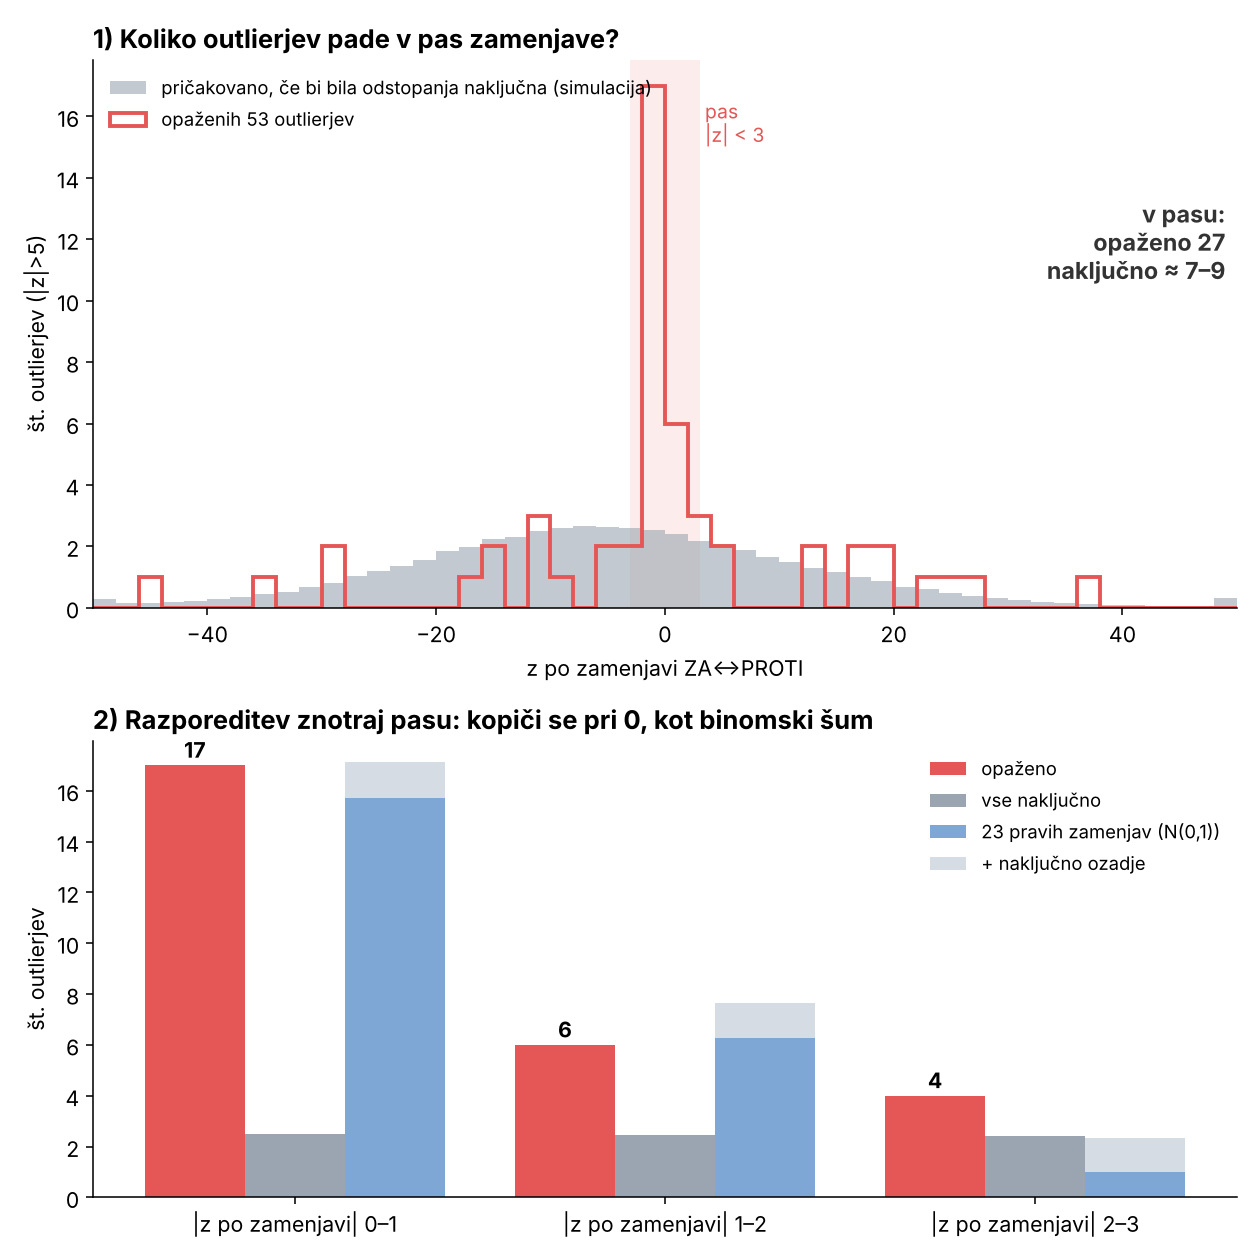
\includegraphics[width=0.64\textwidth]{9_test_pasu.png}
\caption{Zgoraj: $z^{\text{zam}}$ za 53 outlierjev proti simulaciji naključnih odstopanj. Spodaj: razporeditev znotraj pasu.}
\label{fig:pas}
\end{figure}

\subsection{Zakaj resnična posebnost ne pade na zrcalno vrednost}

Resnična posebnost volišča (sestava volivcev, lokalna tema, zmeda pri vprašanju) premakne rezultat za količino, ki ni povezana z oddaljenostjo napovedi od 50~\%. Da bi premik padel na zrcalno vrednost, bi moral biti naključno natanko dvakratna razdalja napovedi od 50~\%: pri napovedi 36~\% točno $+28$ odstotnih točk, pri napovedi 70~\% točno $-40$ točk. Na sliki~\ref{fig:napoved} se to vidi kot zrcalna črta: resnične posebnosti bi se razpršile po ravnini, kot oranžne točke, rdeče pa se nanizajo na črto v obeh smereh in pri različnih razdaljah od 50~\%. To je podpis mehanske operacije s števili, pri kateri dve števili zamenjata mesti.

Enako velja za porazdelitev z debelejšimi repi od predpostavljene in za nenatančnost modela: oboje porazdelitev odstopanj razširi, ne ustvari pa vrha na vrednosti, ki je za vsako volišče drugačna.

\subsection{Volišča v isti stavbi}\label{sec:stavba}

Volivci v isti stavbi so si demografsko zelo podobni, zato bi se resnična posebnost pokazala tudi pri sosednjih voliščih. Pri osmih domnevnih zamenjavah so v isti stavbi še druga volišča. Pri sedmih od njih je objavljeni rezultat od sosednjih volišč oddaljen 15--39 odstotnih točk, rezultat po zamenjavi pa le 0--7 točk:

\begin{center}
\small\setlength{\tabcolsep}{4pt}\begin{tabular}{llrrrl}
\toprule
 & & \multicolumn{4}{c}{delež ZA (\%)} \\
\cmidrule(lr){3-6}
Volišče z domnevno zamenjavo & referendum & objavljeno & po zamenjavi & napoved & sestrska volišča \\
\midrule
Koper~1/22, SEPŠ & preiskava & \textbf{65} & 35 & 36 & 32, 30, 31, 31, 36 \\
Moste-Polje~3/18, Kodeljevo & preiskava & \textbf{65} & 35 & 37 & 37, 31, 34 \\
Vič-Rudnik~4/31, Obrtna zbornica & RTV & \textbf{62} & 38 & 40 & 45 \\
Logatec/30, OŠ 8 talcev & sociala & \textbf{40} & 60 & 60 & 55 \\
Ptuj~2/24, DK Turnišče & sociala & \textbf{31} & 69 & 72 & 69 \\
Žalec~2/37, Dom kulture Braslovče & sociala & \textbf{34} & 66 & 65 & 68 \\
Brežice/8, SIC Brežice & RTV & \textbf{62} & 38 & 37 & 45 \\
Moste-Polje~1/24, OŠ Sostro & preiskava & \textbf{58} & 42 & 45 & 46, 55 \\
\bottomrule
\end{tabular}
\end{center}

Pri prvih sedmih so sestrska volišča pri istem referendumu povsem v skladu z napovedjo ($|z|\leq1{,}7$ pri vseh). Izjema je OŠ Sostro: eno sestrsko volišče se ujema z zamenjavo, drugo pa ima podoben rezultat kot domnevna zamenjava (55~\%). Tam podatki ne ločijo med zamenjavo in lokalno posebnostjo.

\subsection{Velikost volišč in pogostost}

Domnevne zamenjave so na izrazito večjih voliščih. Ker so na velikih voliščih zamenjave lažje zaznavne (manjši šum), jih primerjam le s celicami, kjer bi bila zamenjava zaznavna: mediana 394 proti 258 glasov (Mann-Whitney $p=0{,}004$). Hipoteza ``enaka verjetnost napake na volišče'' je zavrnjena ($p=0{,}05$), hipoteza ``verjetnost sorazmerna s številom glasov'' pa se ujema skoraj popolno ($p=0{,}95$). Stopnja je okoli 9 domnevnih zamenjav na milijon glasov. Ob upoštevanju zamenjav blizu 50~\%, ki jih ni mogoče zaznati, ima okoli 1~\% volišč zamenjavo pri vsaj enem od štirih referendumov. To je istega reda velikosti kot pri reviziji novozelandskih volitev 2023, ki je napake pri vnosu rezultatov odkrila na 0,3--0,7~\% volišč~\cite{oagnz2024}, vendar je primerjava zaradi različnih vrst napak in načinov odkrivanja le okvirna.

Sorazmernost s številom glasov je skladna s človeško napako: na večjem volišču je glasovnic več, štetje traja dlje, rezultati so praviloma sporočeni pozneje in utrujenost je večja. Tudi Ahlbäck in Jablonski~\cite{ahlback2025} sta pri volitvah v Malaviju 2019 ugotovila, da je bila večina popravkov v zapisnikih volišč posledica človeških napak in da njihovo število narašča z zahtevnostjo štetja. Ta razlaga je verjetna, ni pa preverjena, ker podatki ne vsebujejo časa sporočanja rezultatov. Geografskega vzorca ni: zamenjave so razporejene po vseh volilnih enotah in na 21 od 88 okrajev, velikost volišča pa je edini dejavnik, ki statistično pojasni njihovo razporeditev.

Povezava z velikostjo ne more ustvariti zgoščevanja na zrcalni vrednosti. Tudi če ohranimo točno istih 53 celic (iste velikosti volišč in napovedi) in jim namesto objavljenega rezultata pripišemo naključno resnično posebnost, ki da $|z|>5$, bi ob zrcalni vrednosti pričakovali 2,9--3,8 outlierja, opaženih je 17 ($P\approx10^{-9}$).

%=====================================================
\Needspace{12\baselineskip}
\section{Vpliv na rezultate}

Če na 26 označenih voliščih zamenjamo ZA in PROTI, se izid pri nobenem referendumu ne spremeni; delež ZA se premakne za največ 0,04 odstotne točke.

\begin{center}
\small\begin{tabular}{lrrr}
\toprule
Referendum (zmagovalec) & objavljena prednost & po popravku zamenjav & sprememba \\
\midrule
Preiskava (PROTI) & 23\,147 & 23\,409 & $+262$ \\
RTV (PROTI) & 546 & 1\,372 & $+826$ \\
Sociala (ZA) & 194\,705 & 195\,289 & $+584$ \\
Tujci (ZA) & 97\,776 & 98\,466 & $+690$ \\
\bottomrule
\end{tabular}
\end{center}

Slika~\ref{fig:prisp} prikazuje, kako bi popravek posameznega volišča spremenil prednost zmagovalca. Prikaz je pogojen na hipotezo, da so označena volišča res zamenjave; za morebitne lažne zadetke popravka ni. Posamezni popravki imajo različno smer: barvni prednost zmagovalca povečajo, sivi jo zmanjšajo.

\begin{figure}[H]
\centering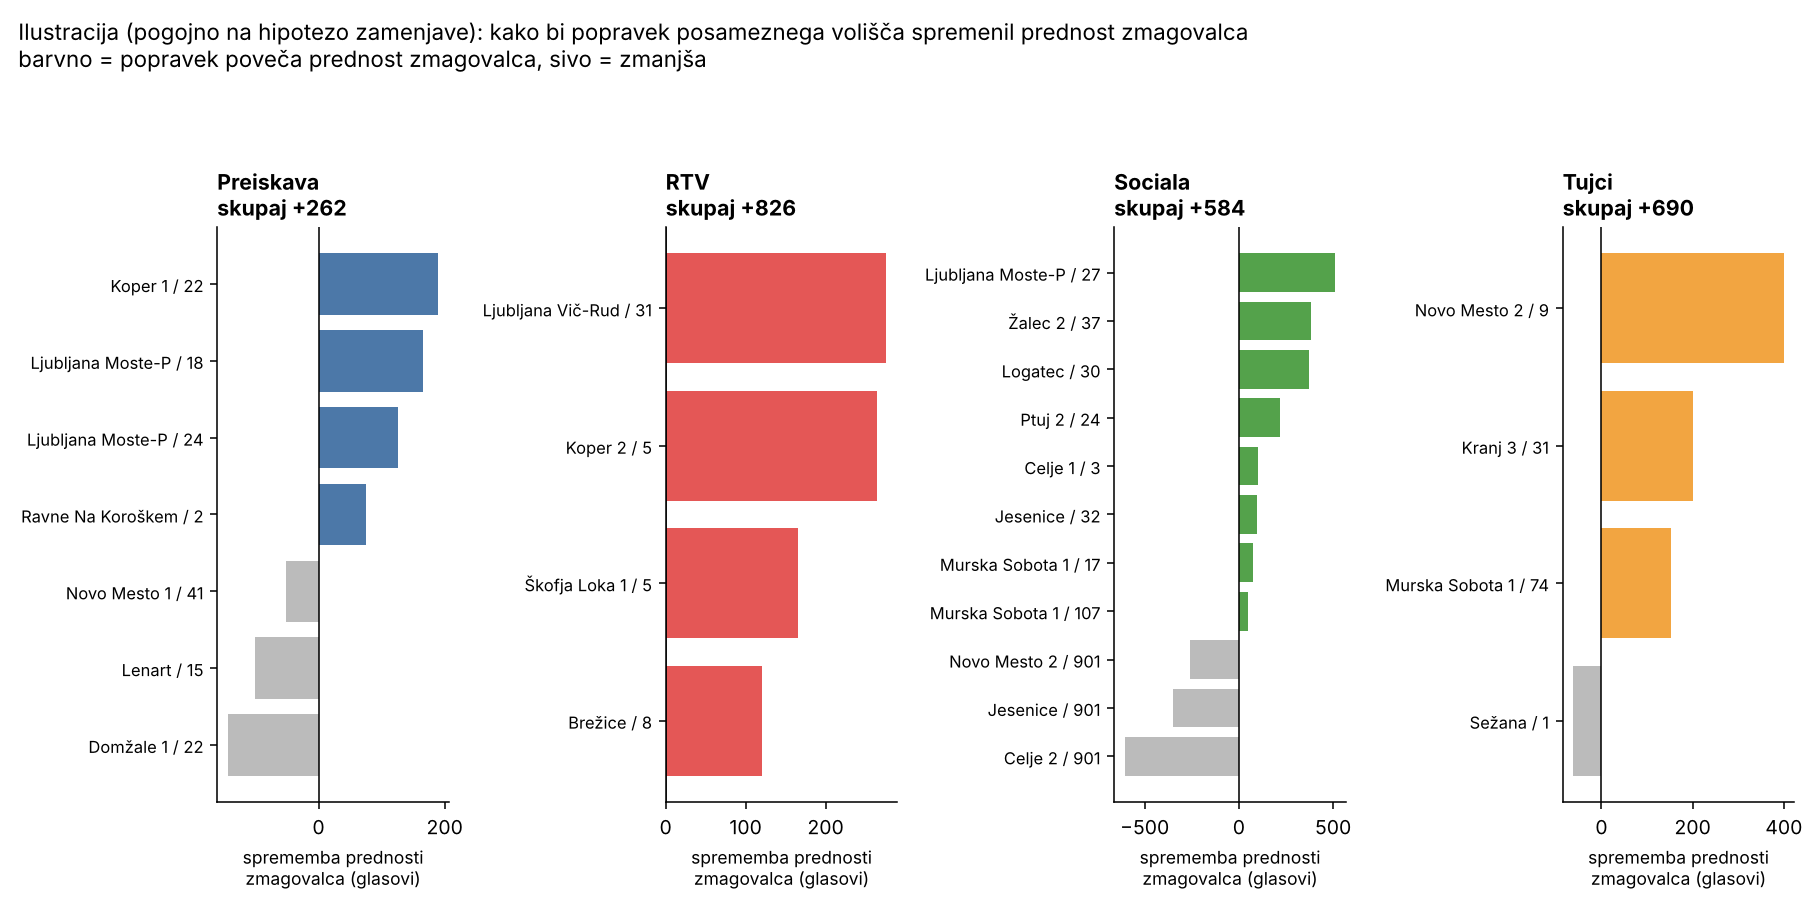
\includegraphics[width=\textwidth]{16_prispevki_volisc.png}
\caption{Sprememba prednosti zmagovalca po popravku posameznega volišča.}
\label{fig:prisp}
\end{figure}

Skupni popravek pri vseh štirih referendumih poveča prednost zmagovalca, kar ni znak pristranskosti. Zamenjava premakne glasove z lokalne večine na lokalno manjšino, zato naključne zamenjave v povprečju izid ``stisnejo'' proti 50~\% in koristijo poraženi strani, ki je pri različnih referendumih različna opcija. Smer je skladna z naključjem. Prirejanje bi sistematično koristilo isti opciji prek vseh referendumov.

%=====================================================
\section{Sklep in preverljivost}

Tudi če presežek outlierjev v celoti pripišemo resničnim lokalnim posebnostim ali porazdelitvi, drugačni od predpostavljene, to ne pojasni zgoščevanja na zrcalni vrednosti. Alternativa bi zahtevala mehanizem, ki da rezultat točno na zrcalni vrednosti napovedi na okoli 20 voliščih z različnimi napovedmi, prizadene le enega od štirih referendumov in se ne pokaže na sosednjih voliščih v isti stavbi. Ostale značilnosti se ujemajo z administrativno napako: smer je skladna z naključjem, zamenjave so razpršene po okrajih, število glasovnic je skladno, vpliv je zanemarljiv in napako je enostavno odkriti iz zapisnika. Statistika sama prevare ne more izključiti, nobena značilnost podatkov pa nanjo ne kaže. Za posamezno volišče rezultat ni dokaz, za obstoj zamenjav kot pojava pa daje močno statistično podporo.

\textbf{Kje bi lahko nastala napaka.} Okrajne volilne komisije rezultate vnašajo iz zapisnikov volilnih odborov in jih primerjajo z zapisniki. Kontroli ``vnos = zapisnik'' in ``veljavne + neveljavne = oddane'' zamenjave rubrik ne ujameta, zato bi lahko napaka, nastala že v zapisniku, ostala tudi v uradnih rezultatih.

\textbf{Preverljivost.} Hipotezo je mogoče preveriti postopno. Najprej se pregledajo tri volišča, pri katerih je zamenjava po modelu najverjetnejša: PGD Bizovik (sociala), Dom kulture Braslovče~II (sociala) in OŠ Mali Slatnik (tujci). Pri vseh treh je verjetnost zamenjave okoli 0,85 (konzervativna ocena). Pregled pomeni primerjavo objave z zapisnikom in, če se ujemata, ponovno štetje glasovnic, saj je napaka lahko nastala že pri vpisu v zapisnik. Če je hipoteza pravilna, je verjetnost, da pri nobenem od treh volišč ne najdemo napake, okoli 0,003, zato bi tak izid hipotezo ovrgel. Če zamenjav ni, bi zrcalno napako lahko našli le po naključju: tudi ob velikodušni predpostavki, da ima 1~\% vseh celic zamenjavo neodvisno od označb modela, je verjetnost vsaj ene najdene napake 0,03, vsaj dveh pa 0,0003. Že ena ali dve potrjeni zamenjavi bi upravičili pregled vseh 26 označenih volišč, pri katerih model napoveduje okoli 20 potrjenih.

\textbf{Omejitve.} Podatki so preliminarni. Pragi ($|z|>5$, $|z^{\text{zam}}|<3$) so hevristični, med zamenjavami je ocenjeno 2--4 lažnih zadetkov. Zamenjave pri deležih blizu 50~\% so nevidne, zato je ocenjeno število spodnja meja.

\textbf{Celotno poročilo} (povezava na prvi strani) vsebuje še podrobnosti modela, seznam vseh 53 outlierjev in dodatne teste. V njem je zgoščevanje na zrcalni vrednosti preverjeno tudi brez izbire pasu (med vsemi outlierji, izbranimi samo po $|z|>5$) in brez modela ozadja, z enakim sklepom: mešani model oceni okoli 22 zamenjav (95-\% IZ 15--30). Skladno oceno da tudi smer odstopanj vseh outlierjev: delež zamenjav med outlierji je ocenjen na 0,5--0,6 iz števila odstopanj v škodo zmagovalca in na 0,25--0,4 iz vsote sprememb prednosti (mešani model: 0,42), vendar ima ta test nizko moč, saj 95-\% interval pri obeh obsega celoten razpon od 0 do 1.

%=====================================================
\vspace*{0pt plus 1filll}
\begin{thebibliography}{9}
\bibitem{wand2001} J.\,N. Wand, K.\,W. Shotts, J.\,S. Sekhon, W.\,R. Mebane Jr., M.\,C. Herron, H.\,E. Brady. The Butterfly Did It: The Aberrant Vote for Buchanan in Palm Beach County, Florida. \emph{American Political Science Review} 95(4):793--810, 2001. \url{https://doi.org/10.1017/S000305540040002X}
\bibitem{mebane2004} W.\,R. Mebane Jr., J.\,S. Sekhon. Robust Estimation and Outlier Detection for Overdispersed Multinomial Models of Count Data. \emph{American Journal of Political Science} 48(2):392--411, 2004. \url{https://doi.org/10.1111/j.0092-5853.2004.00077.x}
\bibitem{ahlback2025} J. Ahlbäck, R.\,S. Jablonski. How to Distinguish Human Error from Election Fraud: Evidence from the 2019 Malawi Election. \emph{British Journal of Political Science} 55, 2025. \url{https://doi.org/10.1017/S0007123425100951}
\bibitem{okfn2014} N.\,E. Kaaber Rasmussen. Open Electoral Data Reveal Errors in Danish Electoral Results. Open Knowledge Denmark, 28.\,5.\,2014. \url{https://dk.okfn.org/index.html?p=127.html}
\bibitem{oagnz2024} Office of the Auditor-General New Zealand. \emph{General Election 2023: Independent review of counting errors}. 7.\,5.\,2024. \url{https://oag.parliament.nz/2024/election-2023/}
\end{thebibliography}

\clearpage
\appendix
\section{Seznam izstopajočih celic}

Seznam vseh 53 celic, ki so izstopajoče v obeh modelih ($|z|>5$), razvrščenih po tipu odstopanja. Stolpci:
\begin{itemize}\setlength{\itemsep}{0pt}
\item \textbf{Okraj, ID, Volišče}: volilni okraj, številka volišča v okraju (901 je predčasno glasovanje) in ime volišča.
\item \textbf{Ref.}: referendum, pri katerem celica izstopa.
\item \textbf{Glasov}: število veljavnih glasov na tem referendumu.
\item \textbf{ZA objav.}: objavljeni delež ZA v \%.
\item \textbf{ZA napov.}: napoved deleža ZA v \% iz ostalih treh referendumov na istem volišču (model brez FE).
\item \textbf{$z$, $z_{\text{FE}}$}: standardizirano odstopanje objavljenega deleža od napovedi v modelu brez oziroma s fiksnimi učinki okraja (enačba~\ref{eq:z}); pozitivno pomeni več ZA, kot je napovedano.
\item \textbf{$z^{\text{zam}}$}: odstopanje, če bi ZA in PROTI zamenjali (enačba~\ref{eq:z}, model brez FE); vrednost blizu 0 pomeni, da se zamenjani rezultat ujema z napovedjo.
\item \textbf{Kor.}: smer odstopanja; ``ZA'' pomeni, da je objavljenih glasov ZA več, kot jih napoveduje model (ali kot bi jih bilo po zamenjavi).
\item \textbf{$\Delta$ZA}: pri domnevni zamenjavi ZA$\leftrightarrow$PROTI razlika objavljeni ZA $-$ pravi ZA (če je zamenjava prava); pri ostalih ($\approx$) grob presežek glasov ZA glede na napoved.
\end{itemize}
Maribor~5/17 je med nepojasnjenimi, ker enojna zamenjava ne zadošča. Objavljeni rezultati se ujemajo s trojno zamenjavo (preiskava, sociala in tujci), po kateri se volišče ujema z okrajem; podrobneje v celotnem poročilu.

{\scriptsize
\setlength{\tabcolsep}{2pt}
\begin{longtable}{>{\raggedright\arraybackslash}p{2.9cm}r>{\raggedright\arraybackslash}p{3.7cm}lrrrrrrlr}
\toprule
Okraj & ID & Volišče & Ref. & Glasov & \shortstack{ZA\\objav.} & \shortstack{ZA\\napov.} & $z$ & $z_{\text{FE}}$ & $z^{\text{zam}}$ & Kor. & $\Delta$ZA \\
\endhead
\midrule
\multicolumn{12}{l}{\textbf{Domnevne zamenjave ZA$\leftrightarrow$PROTI} (26)}\\
\midrule
4005 - Ljubljana Moste-P & 27 & PGD Bizovik & Sociala & 758 & 33 & 68 & -23.7 & -26.6 & -0.5 & PROTI & -256 \\
5005 - Žalec 2 & 37 & Dom kulture Braslovče II & Sociala & 597 & 34 & 65 & -18.5 & -21.2 & +0.7 & PROTI & -191 \\
6003 - Novo Mesto 2 & 9 & OŠ Mali Slatnik & Tujci & 754 & 37 & 62 & -17.8 & -20.2 & +0.7 & PROTI & -200 \\
5003 - Celje 2 & 901 & Predčasno glasovanje & Sociala & 1375 & 61 & 40 & +18.9 & +19.7 & -0.7 & ZA & +303 \\
8010 - Ptuj 2 & 24 & DK Turnišče & Sociala & 278 & 31 & 72 & -17.7 & -19.1 & -0.9 & PROTI & -108 \\
2004 - Koper 1 & 22 & SEPŠ & Preiskava & 323 & 65 & 36 & +14.0 & +16.2 & -0.6 & ZA & +95 \\
3001 - Logatec & 30 & OŠ 8 talcev Logatec & Sociala & 943 & 40 & 60 & -14.5 & -15.2 & -0.1 & PROTI & -185 \\
3006 - Ljubljana Vič-Rud & 31 & Obrtna zbornica Vič & RTV & 568 & 62 & 40 & +11.0 & +14.7 & -0.8 & ZA & +138 \\
4007 - Ljubljana Moste-P & 18 & Park Kodeljevo-Šport Lj. (mala d & Preiskava & 277 & 65 & 37 & +13.0 & +14.4 & -0.7 & ZA & +83 \\
1001 - Jesenice & 901 & Predčasno glasovanje & Sociala & 1004 & 59 & 43 & +11.4 & +14.0 & -1.7 & ZA & +176 \\
4010 - Domžale 1 & 22 & Podružnična šola Blagovica & Preiskava & 260 & 36 & 63 & -12.1 & -13.4 & +0.2 & PROTI & -72 \\
1006 - Kranj 3 & 31 & Srednja vas & Tujci & 404 & 38 & 58 & -10.1 & -13.3 & +2.3 & PROTI & -100 \\
8007 - Lenart & 15 & OŠ Lenart & Preiskava & 152 & 34 & 70 & -12.8 & -13.2 & -1.1 & PROTI & -50 \\
2005 - Koper 2 & 5 & OŠ Elvire Vatovec Prade & RTV & 564 & 62 & 39 & +10.8 & +11.9 & -0.5 & ZA & +132 \\
6003 - Novo Mesto 2 & 901 & Predčasno glasovanje & Sociala & 810 & 58 & 41 & +11.4 & +11.4 & +0.5 & ZA & +130 \\
6005 - Brežice & 8 & (II)SIC Brežice & RTV & 252 & 62 & 37 & +8.3 & +9.6 & +0.5 & ZA & +60 \\
8004 - Murska Sobota 1 & 17 & Vaško-gasilski dom Gederovci & Sociala & 80 & 26 & 64 & -8.3 & -9.5 & +2.1 & PROTI & -38 \\
8004 - Murska Sobota 1 & 74 & Podružnična šola Krog & Tujci & 508 & 43 & 59 & -9.3 & -8.4 & -0.8 & PROTI & -76 \\
1008 - Škofja Loka 1 & 5 & Društvo upokojencev & RTV & 455 & 59 & 44 & +6.5 & +8.6 & -1.3 & ZA & +83 \\
2006 - Sežana & 1 & Avber & Tujci & 123 & 63 & 38 & +6.9 & +8.0 & -0.2 & ZA & +31 \\
8004 - Murska Sobota 1 & 107 & Vaško-gasilski dom Sotina & Sociala & 94 & 37 & 66 & -6.8 & -7.8 & -0.7 & PROTI & -24 \\
1001 - Jesenice & 32 & TVD Partizan Žirovnica & Sociala & 336 & 43 & 60 & -7.5 & -7.6 & -1.3 & PROTI & -48 \\
5002 - Celje 1 & 3 & Sedež MČ Hudinja & Sociala & 405 & 44 & 58 & -6.8 & -7.6 & -0.8 & PROTI & -51 \\
4005 - Ljubljana Moste-P & 24 & OŠ Sostro & Preiskava & 379 & 58 & 45 & +6.8 & +6.9 & -1.9 & ZA & +63 \\
5010 - Ravne Na Koroškem & 2 & Koroška kmetijska zadruga & Preiskava & 384 & 55 & 43 & +6.2 & +6.4 & +1.1 & ZA & +38 \\
6002 - Novo Mesto 1 & 41 & GD Gorenja Stara vas & Preiskava & 90 & 36 & 55 & -5.0 & -5.6 & +2.3 & PROTI & -26 \\
\midrule
\multicolumn{12}{l}{\textbf{Morda zamenjava} (1)}\\
\midrule
3005 - Ljubljana Vič-Rud & 4 & OŠ Vič & Sociala & 439 & 60 & 44 & +7.6 & +5.8 & -2.2 & ZA & $\approx$+87 \\
\midrule
\multicolumn{12}{l}{\textbf{Odstopanje pri več referendumih na istem volišču} (5)}\\
\midrule
4005 - Ljubljana Moste-P & 25 & OŠ Sostro & Preiskava & 471 & 55 & 37 & +10.4 & +10.9 & +4.7 & ZA & $\approx$+82 \\
4005 - Ljubljana Moste-P & 25 & OŠ Sostro & RTV & 471 & 37 & 52 & -6.5 & -6.6 & +4.4 & PROTI & $\approx$-71 \\
4005 - Ljubljana Moste-P & 25 & OŠ Sostro & Tujci & 471 & 73 & 55 & +9.9 & +12.8 & -15.1 & ZA & $\approx$+87 \\
1008 - Škofja Loka 1 & 6 & Zdravstveni dom Škofja Loka & RTV & 510 & 70 & 53 & +7.7 & +9.3 & -10.6 & ZA & $\approx$+87 \\
1008 - Škofja Loka 1 & 6 & Zdravstveni dom Škofja Loka & Tujci & 508 & 70 & 60 & +5.9 & +5.9 & -16.8 & ZA & $\approx$+53 \\
\midrule
\multicolumn{12}{l}{\textbf{Nepojasnjeno} (21)}\\
\midrule
4002 - Ribnica-Dobrepolj & 901 & Predčasno volišče - UE Ribnica & Preiskava & 557 & 24 & 47 & -14.4 & -16.8 & +18.4 & PROTI & $\approx$-127 \\
3005 - Ljubljana Vič-Rud & 19 & OŠ Vrhovci & Sociala & 480 & 28 & 48 & -10.4 & -11.9 & +12.0 & PROTI & $\approx$-98 \\
2005 - Koper 2 & 1 & OŠV Ankaran & Tujci & 460 & 65 & 45 & +10.4 & +11.6 & -5.5 & ZA & $\approx$+91 \\
4004 - Ivančna Gorica & 4 & KD MULJAVA & Preiskava & 451 & 87 & 70 & +10.7 & +11.3 & -34.8 & ZA & $\approx$+79 \\
7009 - Maribor 5 & 17 & OŠ Draga Kobala & Preiskava & 196 & 68 & 42 & +9.6 & +11.2 & -3.8 & ZA & $\approx$+50 \\
1006 - Kranj 3 & 21 & Naklo II & Sociala & 724 & 86 & 75 & +8.3 & +9.8 & -44.1 & ZA & $\approx$+83 \\
3007 - Ljubljana Center & 17 & OŠ Vodmat & Preiskava & 356 & 44 & 27 & +9.4 & +9.6 & +16.4 & ZA & $\approx$+60 \\
5008 - Velenje 2 & 24 & Dom krajanov Pesje & Sociala & 543 & 82 & 67 & +8.3 & +9.4 & -28.4 & ZA & $\approx$+78 \\
7002 - Slovenska Bistric & 39 & Društvo delovnih invalidov & Preiskava & 320 & 47 & 65 & -9.4 & -9.1 & -6.0 & PROTI & $\approx$-60 \\
1008 - Škofja Loka 1 & 11 & Gasilski dom Gosteče & Sociala & 258 & 93 & 74 & +8.3 & +9.3 & -29.0 & ZA & $\approx$+50 \\
4007 - Ljubljana Moste-P & 2 & OŠ Nove Jarše & RTV & 562 & 18 & 34 & -8.1 & -9.0 & +23.5 & PROTI & $\approx$-92 \\
2005 - Koper 2 & 901 & Predčasno glasovanje & Sociala & 879 & 27 & 38 & -7.6 & -8.0 & +24.7 & PROTI & $\approx$-93 \\
3008 - Ljubljana Šiška 1 & 22 & Vrtec Najdihojca & Preiskava & 364 & 28 & 18 & +6.9 & +7.6 & +36.0 & ZA & $\approx$+38 \\
8005 - Murska Sobota 2 & 23 & Večnamenska dvorana Pušča & RTV & 127 & 32 & 13 & +6.6 & +7.0 & +18.4 & ZA & $\approx$+25 \\
4005 - Ljubljana Moste-P & 901 & Predčasno glasovanje & Preiskava & 780 & 37 & 29 & +6.9 & +6.7 & +27.8 & ZA & $\approx$+65 \\
3001 - Logatec & 24 & GD Medvedje Brdo & RTV & 103 & 89 & 65 & +5.1 & +6.4 & -11.6 & ZA & $\approx$+25 \\
1007 - Tržič & 5 & Kovor & Tujci & 732 & 66 & 57 & +5.9 & +6.2 & -15.8 & ZA & $\approx$+64 \\
2007 - Ilirska Bistrica & 901 & Predčasno glasovanje & Tujci & 527 & 44 & 36 & +5.0 & +6.2 & +12.1 & ZA & $\approx$+45 \\
7011 - Maribor 7 & 901 & Predčasno glasovanje & Sociala & 583 & 31 & 40 & -5.5 & -6.0 & +16.5 & PROTI & $\approx$-56 \\
2008 - Postojna & 37 & Dom krajanov Bolk & Tujci & 243 & 69 & 55 & +5.4 & +6.0 & -9.0 & ZA & $\approx$+34 \\
8001 - Lendava & 2 & Medgeneracijski center (Bukovje) & Tujci & 156 & 58 & 74 & -5.8 & -5.5 & -11.2 & PROTI & $\approx$-26 \\
\bottomrule
\end{longtable}
}


\end{document}
